\documentclass[12pt,a4paper]{article}
\usepackage{tikz}
\usetikzlibrary{arrows, arrows.meta}
\usepackage[utf8]{inputenc}
\usepackage{amsfonts}
\usepackage{mathptmx}
\usepackage{float}
\usepackage{graphicx}
\usepackage{hyperref}
\usepackage{setspace}
\usepackage[document]{ragged2e}
\usepackage{fancyhdr}
\usepackage[left=1.5cm,right=1.5cm,top=2.5cm,bottom=2.5cm]{geometry}
\usepackage{gb4e}
\author{Semih Can Aktepe}
\title{COGS543 Assignment 2}

\spacing{1.5}

\pagestyle{fancy}
\fancyhf{}
\lhead{Semih Can Aktepe}
\rhead{\today}
\cfoot{\thepage}

\begin{document}\thispagestyle{empty}
\maketitle
\justify
\textbf{Question 1:}\\
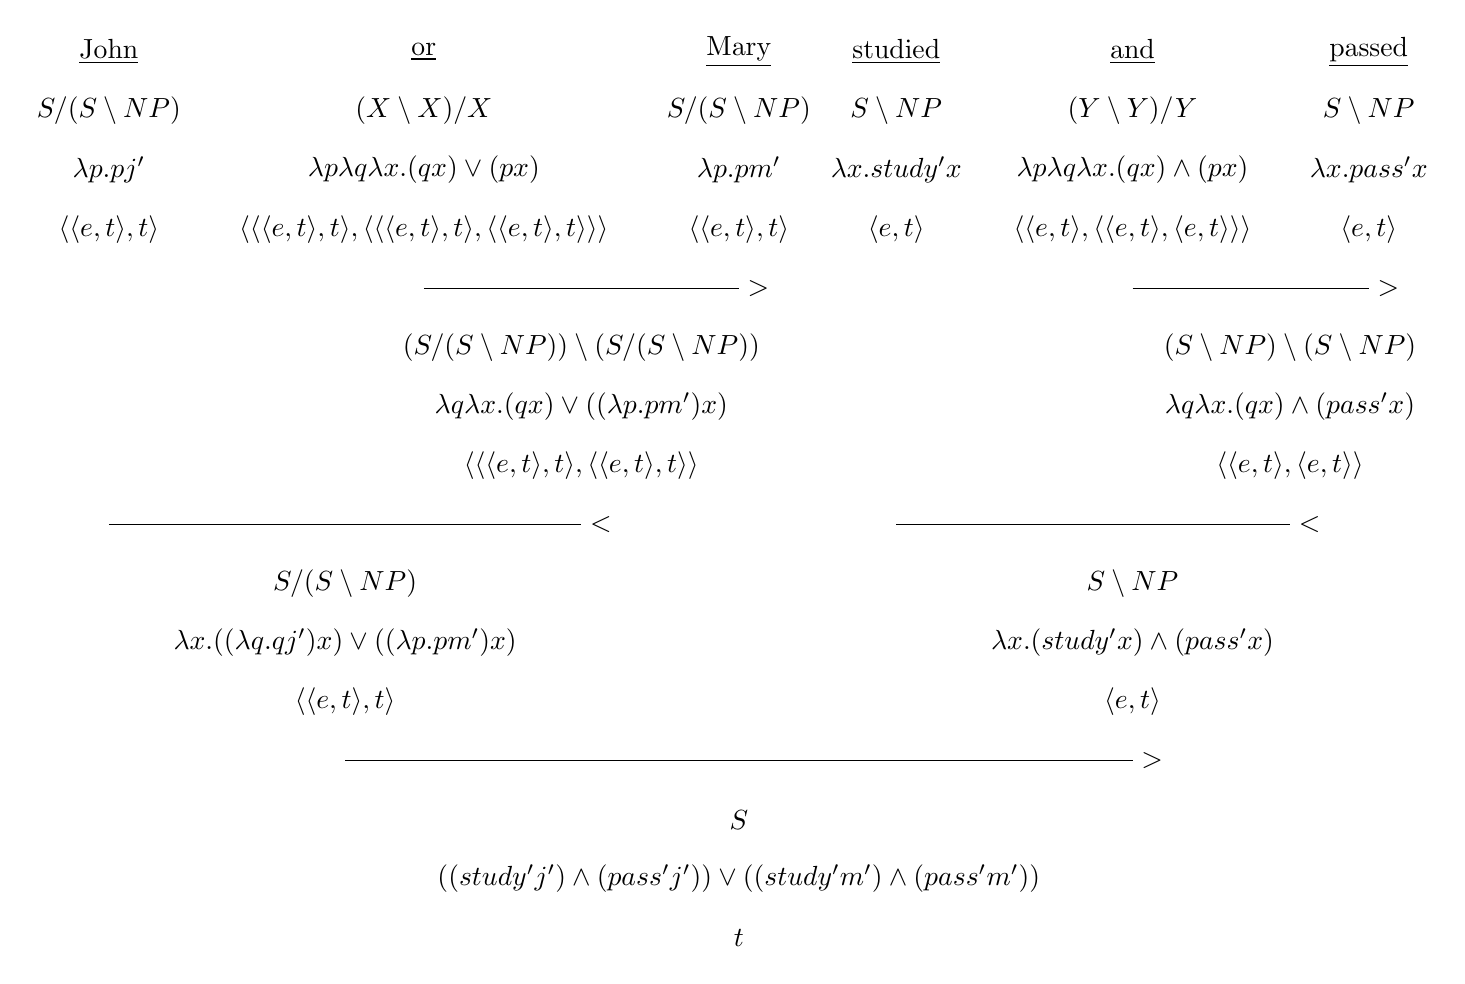
\begin{tikzpicture}
\node at (-1,0){\underline{John}};\node at (-1,-0.75){$S/(S\setminus NP)$};\node at (-1,-1.5){$\lambda p.p j'$};\node at (-1,-2.25){$\langle\langle e,t\rangle, t\rangle$};
\node at (3,0){\underline{or}};\node at (3,-0.75){$(X\setminus X)/X$};\node at (3,-1.5){$\lambda p \lambda q \lambda x.(q x)\vee (p x)$};\node at (3,-2.25){$\langle\langle\langle e,t\rangle, t\rangle,\langle\langle\langle e,t\rangle, t\rangle,\langle\langle e,t\rangle, t\rangle\rangle\rangle$};
\node at (7,0){\underline{Mary}};\node at (7,-0.75){$S/(S\setminus NP)$};\node at (7,-1.5){$\lambda p.p m'$};\node at (7,-2.25){$\langle\langle e,t\rangle, t\rangle$};
\node at (9,0){\underline{studied}};\node at (9,-0.75){$S\setminus NP$};\node at (9,-1.5){$\lambda x.study' x$};\node at (9,-2.25){$\langle e,t\rangle$};
\node at (12,0){\underline{and}};\node at (12,-0.75){$(Y\setminus Y)/Y$};\node at (12,-1.5){$\lambda p \lambda q \lambda x.(q x)\wedge (p x)$};\node at (12,-2.25){$\langle\langle e,t\rangle,\langle\langle e,t\rangle,\langle e,t\rangle\rangle\rangle$};
\node at (15,0){\underline{passed}};\node at (15,-0.75){$S\setminus NP$};\node at (15,-1.5){$\lambda x.pass' x$};\node at (15,-2.25){$\langle e,t\rangle$};

\draw (3,-3)--(7,-3);\node at (7.25,-3){$>$};\draw (12,-3)--(15,-3);\node at (15.25,-3){$>$};
\node at (5,-3.75){$(S/(S\setminus NP))\setminus (S/(S\setminus NP))$};
\node at (5,-4.5){$\lambda q\lambda x.(qx)\vee ((\lambda p.pm')x)$};
\node at (5,-5.25){$\langle\langle\langle e,t\rangle, t\rangle,\langle\langle e,t\rangle, t\rangle\rangle$};

\node at (14,-3.75){$(S\setminus NP)\setminus (S\setminus NP)$};
\node at (14,-4.5){$\lambda q\lambda x.(qx)\wedge (pass'x)$};
\node at (14,-5.25){$\langle\langle e,t\rangle,\langle e,t\rangle\rangle$};

\draw (-1,-6)--(5,-6);\node at (5.25,-6){$<$};\draw (9,-6)--(14,-6);\node at (14.25,-6){$<$};
\node at (2,-6.75){$S/(S\setminus NP)$};
\node at (2,-7.5){$\lambda x.((\lambda q.qj')x)\vee ((\lambda p.pm')x)$};
\node at (2,-8.25){$\langle\langle e,t\rangle, t\rangle$};

\node at (12,-6.75){$S\setminus NP$};
\node at (12,-7.5){$\lambda x.(study'x)\wedge (pass'x)$};
\node at (12,-8.25){$\langle e,t\rangle$};

\draw (2,-9)--(12,-9);\node at (12.25,-9){$>$};
\node at (7,-9.75){$S$};
\node at (7,-10.5){$((study' j')\wedge (pass' j'))\vee ((study' m')\wedge (pass' m'))$};
\node at (7,-11.25){$t$};
\end{tikzpicture}

\vspace{2cm}
\noindent or = $((S/(S\setminus NP))\setminus (S/(S\setminus NP)))/(S/(S\setminus NP))$\\
and = $((S\setminus NP)\setminus (S\setminus NP))/(S\setminus NP)$
\clearpage

\noindent \textbf{Question 2:}\\
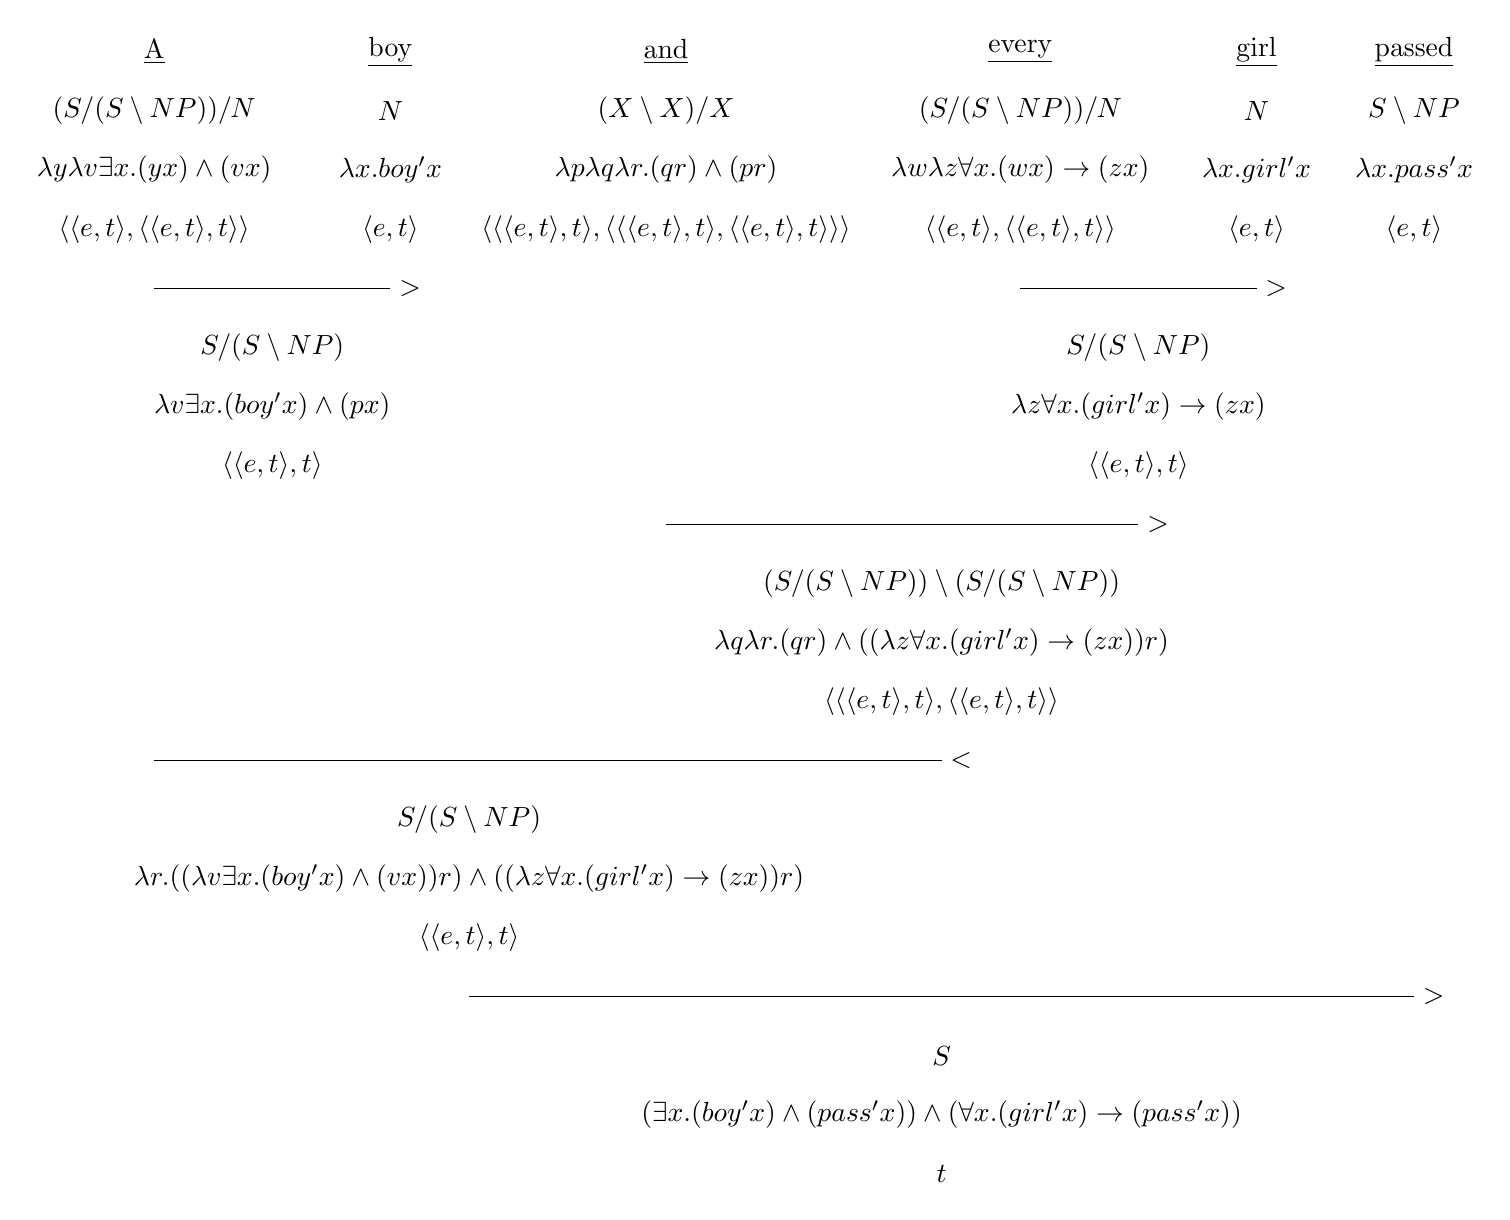
\begin{tikzpicture}
\node at (-1,0){\underline{A}};\node at (-1,-0.75){$(S/(S\setminus NP))/N$};\node at (-1,-1.5){$\lambda y\lambda v\exists x.(yx)\wedge (vx)$};\node at (-1,-2.25){$\langle\langle e,t\rangle,\langle\langle e,t\rangle, t\rangle\rangle$};
\node at (2,0){\underline{boy}};\node at (2,-0.75){$N$};\node at (2,-1.5){$\lambda x.boy'x$};\node at (2,-2.25){$\langle e,t\rangle$};
\node at (5.5,0){\underline{and}};\node at (5.5,-0.75){$(X\setminus X)/X$};\node at (5.5,-1.5){$\lambda p \lambda q \lambda r.(q r)\wedge (p r)$};\node at (5.5,-2.25){$\langle\langle\langle e,t\rangle, t\rangle,\langle\langle\langle e,t\rangle, t\rangle,\langle\langle e,t\rangle, t\rangle\rangle\rangle$};
\node at (10,0){\underline{every}};\node at (10,-0.75){$(S/(S\setminus NP))/N$};\node at (10,-1.5){$\lambda w\lambda z\forall x.(wx)\rightarrow (zx)$};\node at (10,-2.25){$\langle\langle e,t\rangle,\langle\langle e,t\rangle, t\rangle\rangle$};
\node at (13,0){\underline{girl}};\node at (13,-0.75){$N$};\node at (13,-1.5){$\lambda x.girl'x$};\node at (13,-2.25){$\langle e,t\rangle$};
\node at (15,0){\underline{passed}};\node at (15,-0.75){$S\setminus NP$};\node at (15,-1.5){$\lambda x.pass'x$};\node at (15,-2.25){$\langle e,t\rangle$};

\draw (-1,-3)--(2,-3);\node at (2.25,-3){$>$};
\node at (0.5,-3.75){$S/(S\setminus NP)$};
\node at (0.5,-4.5){$\lambda v\exists x.(boy'x)\wedge (px)$};
\node at (0.5,-5.25){$\langle\langle e,t\rangle, t\rangle$};

\draw (10,-3)--(13,-3);\node at (13.25,-3){$>$};
\node at (11.5,-3.75){$S/(S\setminus NP)$};
\node at (11.5,-4.5){$\lambda z\forall x.(girl'x)\rightarrow (zx)$};
\node at (11.5,-5.25){$\langle\langle e,t\rangle, t\rangle$};

\draw (5.5,-6)--(11.5,-6);\node at (11.75,-6){$>$};
\node at (9,-6.75){$(S/(S\setminus NP))\setminus (S/(S\setminus NP))$};
\node at (9,-7.5){$\lambda q\lambda r.(qr)\wedge((\lambda z\forall x.(girl' x) \rightarrow (zx))r)$};
\node at (9,-8.25){$\langle\langle\langle e,t\rangle, t\rangle,\langle\langle e,t\rangle, t\rangle\rangle$};

\draw (-1,-9)--(9,-9);\node at (9.25,-9){$<$};
\node at (3,-9.75){$S/(S\setminus NP)$};
\node at (3,-10.5){$\lambda r.((\lambda v\exists x.(boy' x) \wedge (v x))r)\wedge((\lambda z\forall x.(girl' x) \rightarrow (zx))r)$};
\node at (3,-11.25){$\langle\langle e,t\rangle, t\rangle$};

\draw (3,-12)--(15,-12);\node at (15.25,-12){$>$};
\node at (9,-12.75){$S$};
\node at (9,-13.5){$(\exists x.(boy' x) \wedge (pass' x))\wedge(\forall x.(girl' x) \rightarrow (pass' x))$};
\node at (9,-14.25){$t$};
\end{tikzpicture}

\vspace{2cm}
\noindent and = $((S/(S\setminus NP))\setminus (S/(S\setminus NP)))/(S/(S\setminus NP))$








\end{document}